\documentclass[10pt,letterpaper]{article}
\usepackage{multirow}
\usepackage{cogsci}
\usepackage{pslatex}
\usepackage{amsmath}
\usepackage{amsfonts}
\usepackage{setspace}
\usepackage{apacite}
\usepackage{graphicx}
\usepackage{caption}
\usepackage{subcaption}
\usepackage{etex}
%\usepackage{subfigure}
\usepackage{color}
\usepackage[usenames,dvipsnames,svgnames,table]{xcolor}
\usepackage[usenames,dvipsnames]{xcolor}
\usepackage{tikz}
\usepackage{array}




%\usepackage{todonotes}

\usetikzlibrary{decorations.shapes}
\title{The Funny Thing About Incongruity: A Noisy Channel Model of Puns}
 
 \author{{\large {\bf Justine Kao$^1$} (justinek@stanford.edu)}, {\large {\bf Roger Levy$^2$} (rlevy@ucsd.edu)}, {\large {\bf Noah D.~Goodman$^1$} (ngoodman@stanford.edu)}\\
  $^1$Department of Psychology, Stanford University. $^2$Department of Linguistics, UCSD. }
 
 
%\author{{\large \bf Justine Kao (justinek@stanford.edu)} \\
%  Department of Psychology \\
%  Stanford, USA
%  \AND {\large \bf Noah Goodman (ngoodman@stanford.edu)} \\
%  Department of Psychology \\
%  Stanford, USA
%   \AND {\large \bf Roger Levy (rlevy@ucsd.edu)} \\
%  Department of Linguistics \\
%  UCSD, USA
%  }


\begin{document}

\maketitle

\begin{abstract}
\emph{Researchers showed the robot ten puns, hoping that one of them would make it laugh. Unfortunately, no pun in ten did.}\\

What makes something funny? Humor theorists posit that incongruity---perceiving a situation from different viewpoints and finding the resulting interpretations to be incompatible---contributes to sensations of mirth. In this paper, we use a computational model of sentence comprehension to formalize incongruity and test its relationship to humor in puns. By combining a noisy channel model of language comprehension and standard information theoretic measures, we derive two dimensions of incongruity---ambiguity of meaning and distinctiveness of viewpoints---and use them to predict humans' judgments of funniness. Results showed that both ambiguity and distinctiveness are significant predictors of humor. Moreover, our measures are able to identify specific features of a pun that make it amusing. We show that a probabilistic model of language comprehension can help explain complex social phenomena such as humor.

\textbf{Keywords:} 
Humor; language understanding; noisy channel; probabilistic models; sentence processing
\end{abstract}
\section{Introduction}

Humor plays an essential role in human interactions: it has important positive effects on children's development \cite{frank1989humor}, success in the work place \cite{duncan1990humor}, coping with illness and traumatic events \cite{johnson2002use, gelkopf1996humor}, and marital satisfaction \cite{ziv1989humor}.
Indeed, in a study on gender differences in desired characteristics of relationship partners, both men and women rated sense of humor as more important than physical attractiveness and earning potential \cite{stewart2000sex}. 
In this paper, we are interested in understanding how this fundamental and ubiquitous phenomenon works from the perspective of cognitive science. What makes something funny? How might the defining characteristics of humor shed light on the ways in which the mind processes and evaluates information?

A leading theory of humor posits that incongruity---perceiving a situation from different viewpoints and finding the resulting interpretations to be incompatible---contributes to sensations of mirth \cite{veale2004incongruity, forabosco1992cognitive, mcghee1979humor, martin2007psychology, hurley2011inside}; an idea that dates to Kant's theories about laughter and the sublime \cite{veatch1998theory, forabosco1992cognitive}. Although there is disagreement about whether incongruity alone is sufficient, most theorists accept that incongruity is necessary for producing humor: as Veale (2004) states, ``Of the few sweeping generalizations one can make about humor that are neither controversial or trivially false, one is surely that humor is a phenomenon that relies on incongruity." 
%(dating to Kant's theories about laughter and the sublime \cite{veatch1998theory, forabosco1992cognitive})
However, definitions of incongruity are often ambiguous and difficult to operationalize in empirical research. In this paper, we use a computational model of language understanding to formalize a notion of incongruity and test its relationship to humor. 

Language understanding in general, and particularly humor, relies on rich commonsense knowledge, reasoning, and discourse understanding. To somewhat limit the scope of our task, we focus on applying formalizations of incongruity to a subset of linguistic humor: puns. Writer and philosopher Henri Bergson defined a pun as ``a sentence or utterance in which two ideas are expressed, and we are confronted with only one series of words." This definition highlights the fact that one sentence must evoke two different interpretations in order to be a pun, which aligns with the concept of incongruity as a requisite of humor. 

We develop our model on homophone puns---puns that contain homophone words---because the space of possible interpretations of a homophone pun is relatively constrained and well-defined. An example helps to illustrate: 
\begin{itemize}
\item [] \emph{``The magician got so mad he pulled his hare out."} 
\end{itemize}
This sentence allows for two interpretations:
\begin{itemize}
\item[(a)] The magician got so mad he performed the trick of pulling a rabbit out of his hat.
\item[(b)] The magician got so mad he (idiomatically) pulled out the hair on his head.
\end{itemize}
If the comprehender interprets the word ``hare" as itself, he will arrive at interpretation (a); if he interprets the word as its homophone ``hair," he will arrive at interpretation (b). In other words, the sentence-level differences between interpretations (a) and (b) can be approximated by the two interpretations of the observed word ``hare." In general, distinct interpretations of a homophone pun hinges on one phonetically ambiguous word, allowing the two lexical forms of the homophone word to stand in for competing interpretations of the entire sentence. 

Critically, even though the example we gave was a written pun and the reader sees the word ``hare" explicitly on the page, the ``hair" interpretation is still present and even salient in the context of the sentence. 
%We propose that the reason why two ideas can be communicated through one set of words is because comprehenders maintain uncertainty about the input and consider alternative meanings distinct from what is directly observed. 
Noisy channel models of sentence processing posit that language comprehension is a rational process that incorporates uncertainty about the input at the word level to arrive at sentence-level interpretations that are globally coherent \cite{levy2008noisy, levy2009eye}. This process allows the comprehender to consider multiple word-level interpretations (``viewpoints'') to arrive at more than one interpretation of a sentence, each coherent but potentially incongruous with each other. The notion of incongruity thus fits naturally into a noisy channel model of sentence comprehension.

Our purposes for developing a formal model of linguistic humor are two-fold. First, we wish to formalize the concept of incongruity and test assumptions adopted by leading theories in humor research. Secondly, we aim to show that a noisy channel of language processing allows for flexible context selection and sentence comprehension that gives rise to sophisticated linguistic and social meaning such as humor. 

\section{Model}
Incongruity is a property of the interpretations derived from a sentence.
In order to formalize incongruity we thus first describe a probabilistic model of sentence comprehension.
Our model aims to infer the topic of a sentence (a course representation of its meaning) from the observed words. 
However we take a noisy channel approach, assuming that the comprehender maintains uncertainty over which words reflect the sentence topic and which are noise.
From this model we derive two quantities that may contribute to humor: ambiguity and distinctiveness.
If the resulting interpretation is unambiguous, then no incongruity exists and the sentence is unlikely to be funny. If the resulting interpretation is ambiguous, and furthermore if each interpretation is supported by a distinct topical subset of the sentence (or ``viewpoint''), then the sentence is likely to evoke a sense of incongruity and thus humor. 

Assume our sentence is composed of a vector of content words $\vec w = \{w_1, \dots, w_i, h, w_{i+1}, \dots ,w_n\}$, including a phonetically ambiguous word $h$. 
We will use a simple generative model for $\vec w$ (see Figure~\ref{generativeModel}): given the latent sentence topic $m$, each word is generated independently by first deciding if it reflects the topic (the indicator variable $f_i$), if so it is sampled based on semantic relevance to $m$, if not it is sampled from a fixed unigram prior over words. We thus view the sentence as a mixture of topical and non-topical words. Similar approaches have been used in generative models of language to account for words that serve purposes in a sentence distinct from providing semantic information, such as topic models that incorporate syntax \cite{griffiths2005integrating}. 
Our model is motivated by the important role that semantic priming plays in lexical disambiguation during sentence processing \cite{seidenberg1982automatic, simpson1981meaning, burke1984semantic}; while ignoring the other non-semantic factors of interpretation (which may also be important).

We make the simplifying assumption that the plausible candidate topics $m$ of the sentence will correspond to the potential interpretations of the homophone word $h$, which are themselves constrained by phonetic similarity to two alternatives, $m_1$ and $m_2$. For example, in the magician pun described above, $h$ is the phonetically ambiguous target word ``hare," and  $m_1$ and $m_2$ are the candidate interpretations \emph{hare} and \emph{hair}, respectively. The two potential topics of the sentence can be identified by the two interpretations \emph{hare} and \emph{hair}. This assumption reduces the ill-defined space of sentence meanings to the simple proxy of alternate spellings for phonetically ambiguous words.


%We propose a generative model of sentences in which the latent meaning variable $m$ and a latent indicator variable $\vec f$ are responsible for generating the observed words (see Figure~\ref{generativeModel}). Although the target word $h$ is special in the sense that it constrains the space of interpretations to its homophone meanings $m_1$ and $m_2$, in the model we treat $h$ as a contextual cue similar to other words in its relationship to the latent meaning variable $m$ and indicator variable $f_h$. For simplicity of notation, in the following derivations, $\vec w$ includes the target word $h$, and $\vec f$ includes the indicator variable for $h$. 
%
%Previous research suggests that semantic priming plays an important role in lexical disambiguation during sentence processing \cite{seidenberg1982automatic, simpson1981meaning, burke1984semantic}. As a result, we make a second simplifying assumption that comprehenders use only semantic association information to compute the probabilities of a candidate interpretation. 

%$\vec f$ is a vector of indicator values that determines whether each word in a sentence is in semantic focus. When $f_i = 1$, $w_i$ is in semantic focus and is generated due to semantic relevance to $m$. Otherwise if $f_i = 0$, $w_i$ is simply drawn from a default unigram distribution. Similar approaches have been used in generative models of language to account for words that serve purposes in a sentence distinct from providing semantic information, such as topic models that incorporate syntax \cite{griffiths2005integrating}. For our purposes, the indicator variable allows the model to consider subsets of the sentence as viewpoints that may differentially support the two candidate interpretations $m_1$ and $m_2$. 

\begin{figure}
\centering
\tikzset{decorate sep/.style 2 args=
{decorate,decoration={shape backgrounds,shape=circle,shape size=#1,shape sep=#2}}}
\begin{tikzpicture}
\tikzstyle{place}=[circle,draw,inner sep=2pt,minimum size=0.95cm]
 \tikzstyle{plate}=[rectangle,draw,inner sep=0pt]
 \node[place] (m) at (0,3) {$m$};
 \node[place] (w1) at (-2,1) {$w_1$};
 \node[place] (w2) at (-1,1) {$w_2$};
 \node[place] (h) at (0.5,1) {$h$}; 
 \node[place] (wn) at (2,1) {$w_n$};
 \node[place] (f1) at (-2, -0.5) {$f_1$};
 \node[place] (f2) at (-1, -0.5) {$f_2$};
\node[place] (fh) at (0.5, -0.5) {$f_h$};
\node[place] (fn) at (2, -0.5) {$f_n$};
 %\node[place] (wordsprior) at (0,4.5) {$\wordsprior$};
\draw [->] (m) -- (w1);
\draw [->] (m) -- (w2);
\draw [->] (m) -- (h);
\draw [->] (m) -- (wn);
\draw [->] (f1) -- (w1);
\draw [->] (f2) -- (w2);
\draw [->] (fh) -- (h);
\draw [->] (fn) -- (wn);
\draw[decorate sep={0.3mm}{1.65mm},fill] (-0.41,1) -- (-0.05,1);
\draw[decorate sep={0.3mm}{1.65mm},fill] (-0.41,-0.5) -- (-0.05,-0.5);
\draw[decorate sep={0.3mm}{1.65mm},fill] (1.09,1) -- (1.45,1);
\draw[decorate sep={0.3mm}{1.65mm},fill] (1.09,-0.5) -- (1.45,-0.5);
\end{tikzpicture}
\caption{Generative model of a sentence. Each word $w_i$ is generated based on the sentence topic $m$ if the indicator variable $f_i$ puts it in semantic focus; otherwise it is generated as noise (from a unigram distribution). }
\label{generativeModel}
\end{figure}





Using the above generative model, we can infer the joint probability distribution $P(m, \vec f | \vec w) $ of the sentence topic $m$ and the indicator variables $\vec f$ that determine whether each word is in semantic focus. This distribution can be factorized into:
$$
P(m, \vec f | \vec w) = P(m | \vec w) P(\vec f | m, \vec w) 
$$

We derive a measure from each of the factors $P(m | \vec w)$ and $P(\vec f | m, \vec w)$, which we will call \emph{ambiguity} and \emph{distinctiveness} respectively. Ambiguity means the presence of two similarly likely interpretations, which is required for incongruity because a single unambiguous interpretation rules out incompatible interpretations. Distinctiveness measures the degree to which two interpretations are supported by different viewpoints of the sentence, which we represent as distinct sets of words that are in semantic focus given the two values of $m$. Together, these two measures form our formalization of incongruity. 

\subsubsection{Ambiguity} Let $M$ denote the distribution $P(m | \vec w)$, a binomial distribution over the two meaning values $m_1$ and $m_2$ given the observed words. If the entropy of this distribution is low, this means that the probability mass is concentrated on only one meaning, and the alternative meaning is unlikely given the observed words. If entropy is high, this means that the probability mass is more evenly distributed among $m_1$ and $m_1$, and the two interpretations are similarly likely given the contexts. The entropy of $P(m | \vec w)$ is thus a natural measure of the degree of ambiguity present in a sentence. We compute $P(m | \vec w)$ as follows:
\begin{align}
P(m | \vec w) &= \sum_{\vec f} P(m, \vec f | \vec w) \\
&\propto \sum_{\vec f} P(\vec w | m, \vec f) P(m) P(\vec f) \\
&= \sum_{\vec f} \bigg (P(m)P(\vec f)\prod_i P(w_i | m, f_i) \bigg)
\end{align}
%From Bayes' theorem, this is proportional to the following:
%$$
%\sum_{\vec f} P(\vec w | m, \vec f) P(m) P(\vec f)= \sum_{\vec f} \bigg (P(m)P(\vec f)\prod_i P(w_i | m, f_i) \bigg)
%$$
From the generative model, 
\[
    P(w_i | m, f_i) = 
\begin{cases}
    P(w_i),& \text{if } f=0\\
    P(w_i | m), &\text{if } f=1\\
\end{cases}
\]
Once we derive $P(m | \vec w)$, we then compute its entropy as a measure of ambiguity.

\subsubsection{Distinctiveness} We next turn to the distribution over focus sets, given sentence topic. This may be computed as follows:
$$ 
P(\vec f | m, \vec w) \propto P(\vec w | m, \vec f) P(\vec f | m)
$$
Since $\vec f$ and $m$ are independent, $P(\vec f | m) = P(\vec f)$. We assume a uniform probability that each words is in focus.

Let $F_1$ denote the distribution $P(f | m_1, \vec w)$ and $F_2$ denote the distribution $P(f | m_2, \vec w)$. $F_1$ and $F_2$ represent the distributions over semantic focus sets assuming the sentence topic $m_1$ and $m_2$, respectively. We use a symmetrized Kullback-Leibler divergence score $D_{KL}(F_1 || F_2) + D_{KL}(F_2 || F_1)$ to measure the distance between $F_1$ and $F_2$. This score measures how ``distinct" the semantic focus sets are given $m_1$ and $m_2$. A low KL score would indicate that meanings $m_1$ and $m_2$ are supported by similar subsets of the sentence; a high KL score would indicate that $m_1$ and $m_2$ are supported by distinct subsets of the sentence. 

 %Once we derive $P(\vec f | m_1, \vec w)$ and $P(\vec f | m_2, \vec w)$, we compute its symmetrised KL divergence as a measure of distinctiveness.

\section{Evaluation}
By generating a large corpus of sentences involving the same words and measuring subjective funniness of each sentence we can evaluate the contribution of each of our quantitative measures, ambiguity and distinctiveness, to humor.
%We have described a generative model of sentences that incorporates the idea of semantic focus sets and used the model to derive two measures that formalize incongruity. 
We evaluate our model and measures on a set of $235$ sentences, consisting of $65$ puns, $40$ ``de-punned" control sentences that are matched with a subset of the puns, and $130$ non-pun control sentences that match the puns in containing the same phonetically ambiguous words.  


\subsection{Materials}
We selected $40$ pun sentences from a large collection of puns on a website called �Pun of the Day,� which contains over one thousand puns. Puns were selected such that the ambiguous item is a single phonetically ambiguous word, and no two puns in the collection have the same ambiguous item. To obtain more homophone pun items, a research assistant generated an additional $25$ pun sentences based on a separate list of homophone words.

We constructed $40$ sentences to be minimally different from the pun sentences that we collected from ``Pun of the Day," which we will call de-punned sentences. A second research assistant who was blind to the hypothesis was asked to replace one word in each of the pun sentences (without changing the homophone word itself) so that the sentence is still grammatical but is no longer a pun. This resulted in sentences that differed from the pun sentences by one word each.

The $130$ non-pun sentences were chosen to match each pun sentence on its ambiguous word as well as the alternative homophone. The sentences were taken from an online version of Heinle's Newbury House Dictionary of American English (http://nhd.heinle.com/). We selected sample sentences included in the definition of the homophone word. This design ensured that puns, de-punned, and non-pun sentences all contain the same set of phonetically ambiguous words. Figure~\ref{exampleSentences} shows example sentences from each category.\\\\
\begin{figure}[h]
\begin{tabular}{| l | l |}\hline
\textbf{Type} & \textbf{Example} \\\hline
Pun & The magician got so mad he pulled his hare out. \\
De-pun & The professor got so mad he pulled his hare out.\\
Non-pun& The hare ran rapidly across the field.\\
Non-pun& Some people have lots of hair on their heads.\\\hline
\end{tabular}
\caption{Example sentences from each category}
\label{exampleSentences}
\end{figure}

\subsection{Human ratings of semantic relatedness}
As described in the model section, computing our measures requires the prior probabilities of meanings $P(m)$, the prior probabilities of words $P(w)$, and the conditional probabilities of each word in the sentence given a meaning $P(w | m)$. While we computed $P(w)$ and $P(m)$ directly from the Google unigram corpus, $P(w | m)$ is difficult to obtain through corpora due to data sparsity. 
However, since each meaning we consider has a single word as proxy, we may approximate $P(w | m)$ using an empirical measure of the semantic relatedness between $w$ and $m$, denoted $R(c, m)$. We use $R(c, m)$ as a proxy for point wise mutual information between $c$ and $m$, defined as follows:
$$
R(w, m)= {\log \frac{P(w, m)}{P(w)P(m)}} = \log \frac{P(w | m)}{P(w)} = \log P(w | m) - \log P(w)
$$
With the proper substitutions and transformations, 
$$
P(w | m) = e^{R(w, m)} P(w)
$$

\begin{figure*}[t]
\mbox{
\begin{subfigure}{0.45\textwidth}
\scalebox{0.4}{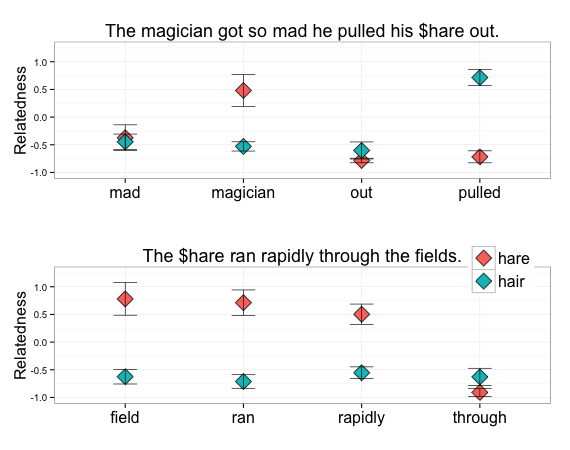
\includegraphics{Plots/relatedness_example.png}}
\subcaption{Relatedness of word pairs in example pun and non-pun}
\end{subfigure}
\begin{subfigure}{0.29\textwidth}
\scalebox{0.4}{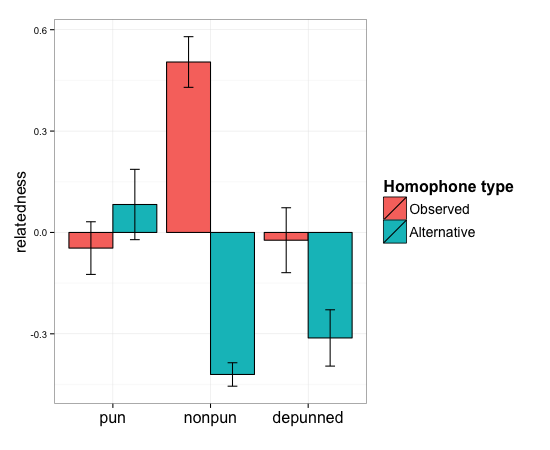
\includegraphics{Plots/ave_relatedness.png}}
\subcaption{Average relatedness of word pairs}
\end{subfigure}
\begin{subfigure}{0.31\textwidth}
\scalebox{0.4}{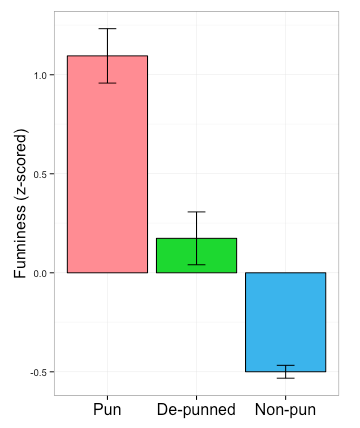
\includegraphics{Plots/ave_funniness.png}}
\subcaption{Average funniness of sentences}
\end{subfigure}
}
\caption{Analyses of human ratings}
\label{ratings_analyses}
\end{figure*}
To obtain $R(w, m)$ for each of the words $w$ in the stimuli sentences, we recruited $200$ subjects on Amazon's Mechanical Turk to rate distinct word pairs on their semantic relatedness. Function words were removed from the sentences, and the remaining words were paired with each of the interpretations of the homophone sequence (e.g., ``magician" and ``hare" is a legitimate word pair, as well as ``magician" and ``hair"). This resulted in $1460$ distinct word pairs. Each subject saw $146$ pairs of words in random order and were asked to rate how related each word pair is using a scale from $1$ to $10$. The average split-half correlation of the relatedness ratings was $0.916$, indicating that semantic relatedness was a reliable measure. 

Figure~\ref{ratings_analyses} (a) shows the relatedness of each content word with the two homophone interpretations for two example sentences. In the top sentence, which is a pun, the word ``magician" is rated as significantly more related to ``hare" than it is to ``hair", while the word ``pulled" is rated as significantly more related to ``hair" than it is to ``hare." In the bottom sentence, which is a non-pun, all words except the neutral word ``through" are more related to the word ``hare" than to ``hair." 

Figure~\ref{ratings_analyses} (b) shows the average relatedness ratings of words and the two homophone interpretations across the three types of sentences. In pun sentences, the average relatedness of words to the two homophone interpretations are roughly equivalent. In the de-punned sentences, the average relatedness of words to the observed homophone is significantly lower than to the alternative homophone. In the non-pun sentences,the average relatedness of words to the observed homophone is significantly higher than to the alternative homophone. These analyses suggest that relatedness ratings for the two candidate meanings capture the presence or absence of multiple interpretations in puns, de-punned sentences, and non-puns. It further supports our model's prediction that ambiguity of meaning and the distinctiveness of supporting context words can help distinguish among the three types of sentences.

\subsection{Human Ratings of Funniness}
We obtained funniness ratings of the $235$ sentences from $100$ subjects on Amazon's Mechanical Turk. Each subject read roughly $60$ sentences in random order, counterbalanced for the sentence types, and rated each sentence on funniness and correctness. The average split-half correlation of funniness ratings was $0.83$. Figure~\ref{ratings_analyses} (c) shows the average funniness ratings of puns, de-punned, and non-pun sentences. Pun sentences are rated as significantly funnier than de-punned sentences, and de-punned sentences are rated as significantly funnier than non-pun sentences ($F(2, 232) = 415.3, p < 0.0001$). Figure~\ref{ratings_analyses} (b) and Figure~\ref{ratings_analyses} (c) together suggest that the balance of relatedness between the two interpretations is a predictor of funniness.

\section{Results}
Following the derivations described in the model section and using the relatedness measures described above, we computed an ambiguity and distinctiveness value for each of the $235$ sentences. As predicted, ambiguity differs significantly across sentence types ($F(2, 232) = 11.94, p < 0.0001 $) and correlates significantly with human ratings of funniness across the $235$ sentences ($r = 0.27, p < 0.0001$). Furthermore, distinctiveness scores differ significantly across sentence types as well ($F(2, 232) =  5.76, p < 0.005$) and correlates significantly with human ratings of funniness ($r = 0.21, p < 0.005$).
\begin{table}[t]
\centering
\begin{tabular}{| l | r | r | l |}\hline
& {Estimate} & Std. Error & {p value} \\\hline
Intercept & $-0.687$ & $0.140$ & $< 0.0001$ \\
Ambiguity & $1.011$ & $0.193$ & $< 0.0001$\\
Distinctiveness & $0.237$ & $0.054$ & $< 0.0001$\\\hline
\end{tabular}
\caption{Regression model for funniness ratings}
\label{coefficients}
\end{table}

A linear regression model showed that both ambiguity and distinctiveness are significant predictors of funniness. Together, the two predictors capture a modest but significant amount of the variance in funniness ratings ($F(2,232) =19.6,  R^2 = 0.137, p < 0.001$) (see Table~\ref{coefficients}). Using both ambiguity and distinctiveness as dimensions that formalize incongruity, we can distinguish among puns, non-puns, and de-punned sentences, as shown in Figure~\ref{ellipse}. Figure~\ref{ellipse} shows the standard error ellipses for each of the three sentence types in the two-dimensional space of ambiguity and distinctiveness. Although there is a fair amount of noise in the predictors (likely due to simplifying assumptions, the need to use empirical measures of relatedness, and the inherent complexity of humor) we see that pun sentences tend to cluster at a space with higher ambiguity and distinctiveness. While de-punned sentences are also fairly high on ambiguity (e.g. it is ambiguous whether the word ``hare" in ``The professor got so mad he pulled his hare out" should be interpreted as \emph{hair}), they tend to have lower distinctiveness measures. Non-pun sentences score the lowest on ambiguity and have moderate distinctiveness measures.

\begin{table*}[!htbp]
\centering
\hfill{}
\begin{tabular}{|c|c|l|l|c|c|r|}
\hline
\textbf{$m1$}& \textbf{$m2$} & \textbf{Type} & \textbf{Sentence and Semantic Focus Sets}& \textbf{Amb.} & \textbf{Disj.} & \textbf{Funniness}\\\hline
\multirow{4}{*}{{\color{Red} hare}} & \multirow{4}{*}{{\color{Emerald} hair}} & Pun & The \textbf{{\color{Red}magician}} got so mad he \textbf{{\color{Emerald}pulled}} his \textbf{{\color{Red}hare}} out. & $0.378$ & $2.291$ & $1.714$\\
&&De-pun & The professor got so mad he \textbf{{\color{Emerald} pulled}} his \textbf{{\color{Red} hare}} out. & $0.048$ & $1.832$ & $-0.103$\\
&&Non-pun & The \textbf{{\color{Red} hare}} \textbf{{\color{Red} ran}} \textbf{{\color{Red} rapidly}} through the \textbf{{\color{Red} fields}}. & $0.447$ &	$1.677$ &	$-0.400$\\
&&Non-pun & Most \textbf{{\color{Emerald} people}} have \textbf{{\color{Emerald} lots}} of \textbf{{\color{Emerald} hair}} on their \textbf{{\color{Emerald} heads}}. & $0.0004$ &	$2.807$ & $-0.343$ \\\hline
\multirow{4}{*}{{\color{Red} tiers}} & \multirow{4}{*}{{\color{Emerald} tears}} & Pun & It was an \textbf{{\color{Emerald} emotional}} \textbf{{\color{NavyBlue} wedding}}. Even the \textbf{{\color{Red} cake}} was in \textbf{{\color{Red} tiers.}} & $0.612$ & $2.311$ & $1.541$\\
&&De-pun & It was an \textbf{{\color{Emerald} emotional}} \textbf{{\color{NavyBlue} wedding}}. Even the \textbf{{\color{Emerald} mother-in-law}} was in \textbf{{\color{Red} tiers}}. & $0.189$ & $1.802$ &	$0.057$ \\

&&Non-pun & \textbf{{\color{Red} Boxes}} are \textbf{{\color{Red}stacked}} in \textbf{{\color{Red} tiers}} in the warehouse. & $0.194$ & 	$2.089$ &	$-0.560$\\

&&Non-pun & \textbf{{\color{Emerald} Tears}} ran down her \textbf{{\color{Emerald} cheeks}} as she watched a \textbf{{\color{Emerald} sad}} \textbf{{\color{Emerald} movie}}.& $0.0003$	& $3.283$ &	$-0.569$ \\
\hline
\end{tabular}
\hfill{}
\caption{Semantic focus sets of example sentences. Words in red are in semantic focus with $m_1$; green with $m_2$; blue with both.}
\label{focusExamples}
\end{table*}

\begin{figure}[t]
\scalebox{0.44}{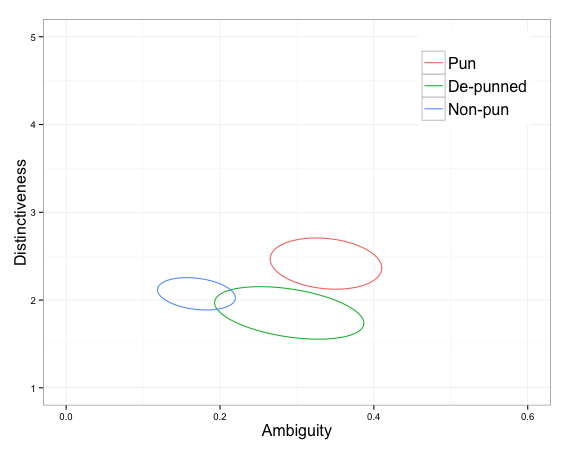
\includegraphics{Plots/ambiguity_distinctiveness_ellipse.png}}
\caption{Standard error ellipses of ambiguity and distinctiveness across sentence types}
\label{ellipse}
\end{figure}

\begin{figure}[t]
\scalebox{0.44}{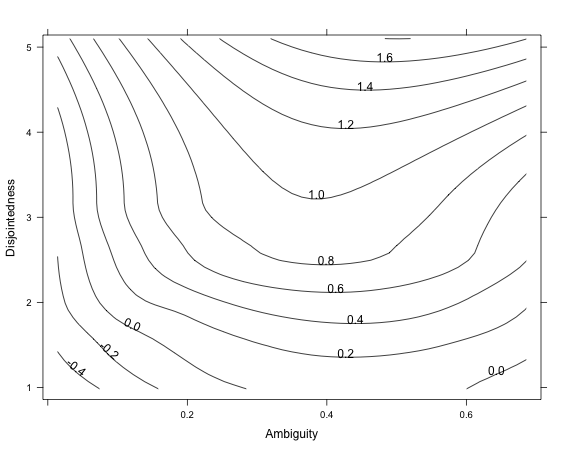
\includegraphics{Plots/contour_plot.png}}
\caption{Ambiguity and disjointedness with funniness contours}
\label{contour}
\end{figure}

Figure~\ref{contour} shows the funniness contours in the two-dimensional ambiguity-distinctiveness space smoothed using a 2-D Loess regression. Not only do the three types of sentences differ along the two dimensions, but sentences become funnier as they increase in ambiguity and distinctiveness. These results suggest that our probabilistic model of language and measures of incongruity capture an important aspect of humor in pun sentences.

Beyond predicting the funniness of a sentence, our model can also tell us which particular features of a pun make it amusing. By finding the most likely semantic focus sets $\vec f$ given each latent meaning variable $m$ and the observed words, we can identify words in a funny sentence that are critical to producing incongruity and humor. Table~\ref{focusExamples} shows the most likely semantic focus sets given each meaning for two groups of sentences. Sentences in each group contain the same pair of candidate meanings for the target word $h$. However, they differ in measures of ambiguity, distinctiveness, and funniness.  Words in the most likely focus sets given $m_1$ are in red; words in the most likely focus sets given $m_2$ are in green; and words in the most likely focus sets of both meanings are in dark blue. We observe that visually, the two pun sentences (which are significantly funnier) have more distinctive and balanced sets of focus words for each meaning than other sentences in their groups. De-punned sentences tend to have fewer words in support of $m_1$, and non-pun sentences tend to have no words in support of the interpretation that was not observed. Moreover, imagine if you were asked to explain why the two pun sentences are funny. The colorful words in each pun sentence---for example, the fact that magicians tend to perform magic tricks with hares, and people tend to be described as pulling out their hair when angry---are what one might intuitively use to explain why the sentence is a pun. Our model thus provides a natural way of not only formalizing incongruity and using it to predict when a sentence is a pun, but also to explain what aspects of a given pun make it funny. 
\section{Discussion}
In this paper, we showed that rich social and linguistic meaning can arise from a very basic model of normal sentence comprehension. We described a probabilistic model of sentence comprehension that uses noisy channel assumptions and semantic association to compute the meaning of a phonetically ambiguous word. Based on this general model of language understanding, we successfully derived predictors of humor in sentences that contain phonetically ambiguous words. 

Researchers in artificial intelligence have argued that computers should be able to generate and detect humor in order to interact with humans more naturally and effectively \cite{mihalcea2006learning}. However, most of the work in computational humor has focused either on utilizing joke-specific templates and schemata \cite{binsted1996machine, kiddon2011s} or identifying surface linguistic features that strongly predict humorous intent \cite{mihalcea2006learning, semantic2010}. The former type of studies is restricted to identifying jokes with a very specific format and structure, and the latter type falls short of testing or building upon more general theories of humor. Our work moves beyond these two approaches and directly utilized a model of general sentence comprehension to identify humorous texts. This approach allows us to apply similar modeling paradigms to explain other types of humor beyond homophone puns. For example, the ambiguity and distinctiveness of longer jokes can be similarly formalized given a way of modeling candidate interpretations and their interactions with context.

Although humor is complex and our task in this paper is limited in scope, we believe that it represents an important step towards developing models of language that can explain complex phenomena such as humor. We hope that our work contributes to research in humor theory, computational humor, and language understanding, such that some day we can understand what makes us laugh and build robots that appreciate the wonders of word play.

\section{Acknowledgments}
We thank Stu Melton and Mia Polansky for helping create and prepare part of the materials used in this paper.

\bibliographystyle{apacite}

\setlength{\bibleftmargin}{.125in}
\setlength{\bibindent}{-\bibleftmargin}

\bibliography{pun_bib}


\end{document}
